% Chapter 2
\newcommand{\systemname}[0]{VideoNote}

\chapter{Navigating Lecture Videos} % Chapter title

\label{ch:visualtranscript} % For referencing the chapter elsewhere, use

%----------------------------------------------------------------------------------------
How viewers watch videos depends on the content of the video and the viewers'
needs. For example, watching a film in a theater is a very different experience
from watching a video tutorial on YouTube about how to cook brussel sprouts.
Even for a same video, someone who is watching it for the first time may have a
different approach from someone who has seen the video previously and is
watching again only to review. In this chapter, we focus on the scenario of
watching lecture videos. \\

Lecture videos are growing in popularity through Massive Open Online Courses
(MOOCs) and flipped classroom models.
However, learning with these videos using existing video player interfaces can
be challenging. Viewers cannot digest the lecture material at their
own pace, and it is also difficult to search or skim the content. For these and other
reasons, some viewers prefer lecture notes or textbooks to videos.\\

To address these limitations, we design \textbf{\systemname}, a readable
interface for lecture videos that resmebles lecture notes with figures and text.
\systemname\ combines visuals presented in the lecture
with its transcript text. To generate a \systemname, we first segment the visual content
of a lecture into a set of discrete \emph{visual entities} that correspond to equations, figures, or lines of text. Then, we analyze
the temporal correspondence between the transcript and the visuals to determine their relationships. Finally, based on the inferred relationships, we arrange the text and visuals into a hierarchical and linear layout. \\

We compare our interface with a standard video player, and a state-of-the-art interface designed specifically for 
lecture videos. User evaluation suggests that users prefer \systemname\ for the task of learning and that \systemname\
facilitates browsing and searching in lecture videos.

%----------------------------------------------------------------------------------------

\section{Introduction}
Despite the increasingly important and broad role of lecture videos in education, learning from such videos poses some challenges. 
%
It is difficult for viewers to consume video content at their own pace~\cite{chi2012mixt}.
%
To skip quickly through familiar concepts or slowly review more difficult material, the viewer must interrupt playback and scrub back-and-forth in the timeline.
%
It is also difficult to find specific information in a video. While scrubbing allows users to browse the visual information in the lecture, it is not effective for skimming the audio content, which often includes critical explanations and context that accompany the visuals. As an alternative, some platforms (e.g., Khan Academy and YouTube) provide synchronized transcripts that allow users to click on a phrase and play the video at that location. However, skimming the transcript for relevant content can also be challenging since the text is not structured, and viewers must click on various parts of the text to see the corresponding visuals. 
%
Finally, it is hard to get a quick overview of the lecture content without watching the entire video. 
For these and other reasons, some people prefer static learning materials such as textbooks or printed lecture notes over videos.\\

Inspired by lecture notes, we present \systemname, a readable interface for both the visual and audio content of a lecture video that facilitates reviewing, browsing and navigation. 
%
We focus on blackboard-style lectures that show a (possibly infinite) blackboard where the instructor writes down by hand the content of the lecture. \systemname s aggregate the full lecture content in a structured format where visual information is segmented and grouped with the corresponding narration text. For example, Figure~\ref{Fig:teaser}(b) shows our automatically generated output for a math lecture that interleaves verbal explanations with the corresponding equations written on the board. 
%
By default, \systemname s hide redundant information to show a compact representation of the content that viewers can expand interactively to show relevant details (Figure~\ref{Fig:teaser}(c)). 
%
Presenting video content in this manner allows users to review the lecture at their own pace while getting both the visual and textual information in a readable, skimmable format.
%
\systemname s is also linked to the video such that clicking on the text or the visuals plays the video from the corresponding location.
%
In this respect, \systemname s offer many of the benefits of traditional static media, such as textbooks and lecture notes, while also giving viewers direct access to the video content.\\

There are two main challenges in transforming a video and its transcribed audio into a \systemname : (1) visuals, which are drawn progressively on the board, must be discretized into  a set of meaningful figures, and (2) such figures and text representing the audio content must be organized into a compact, structured format that emphasizes the relationships between the two channels of information.
%
To segment the visuals into meaningful figures, we propose a dynamic programming approach that takes into account both the spatial layout of strokes and the time when they were drawn. We further time-align the transcript with the audio and use this alignment to establish correspondences between the visuals and the text. Finally, we use the visual-text correspondence to detect redundant information and arrange the content in a compact, sequential layout where the text is organized into readable paragraphs.\\

We evaluate our approach with a user study that compares \systemname\ with a baseline transcript-based video player, and an existing, state-of-the-art visual-based video player developed by Monserrat et al \cite{monserrat2013notevideo}. We measure performance on summarization and search tasks, and observe how the participants interact with the interfaces. We find that \systemname\ is an effective interface for studying lecture videos. Specifically, users performed best using \systemname\ for search tasks involving text. Users noted that \systemname\ helped them to get a quick overview of the video including the details conveyed only through the text, and to efficiently focus on parts of interest. They also found the structured text easier to read and connect to relevant visuals than the baseline text-only transcript. In a post-study survey, users strongly preferred our interface for learning over the other two interfaces.
%----------------------------------------------------------------------------------------
\section{Previous Work}
%
\subsection{Video Visualization}
There is a large body of work that aims to automatically summarize videos to facilitate navigation and browsing, but most research focuses on live action footage which is very different from educational videos.  Recent survey papers \cite{truong2007video,borgo2011survey} comprehensively review these techniques, which can be broadly divided into two classes according to their output: \textit{video skims} and \textit{still-image abstracts}. \\
%
Video skims \cite{he1999auto,ekin2003automatic,ngo2005video,lu2013story} summarize a longer video with a shorter video, usually consisting of segments extracted from the original video. These skims retain audio and motion elements and are especially useful for understanding dynamic scenes, but they are less suitable for conveying the dense, static information of blackboard-style lectures. \\
%
Still-image based methods~\cite{uchihashi1999video,barnes2010video,hwang2006cinema,boreczky2000interactive}
primarily focus on conveying the visual content of a
video in static form through a collection of salient images extracted from the video.~\cite{christel2002collages} and~\cite{pickering2003anses} developed a still-image based method specific to news stories that combines text and images into summaries.\\
%
Most relevant to our work is~\cite{choudary2007summarization}, which summarizes blackboard-style lectures by creating a panoramic frame of the board. In addition to the visual content presented on the board, our interface includes the audio content and therefore maintains the sequence of the lecture and makes textual content directly accessible as well.\\

\subsection{Tools for Online Lecture Videos}
\cite{kim2014data} uses interaction data collected from MOOC platforms to introduce a set of techniques that augment existing video interface widgets. For lecture videos based on slides, \cite{li2000browsing} use separate slides to automatically generate table-of-content overviews. These works \textit{annotate} the original video with useful data to facilitate navigation, but do not reformat the video content. \cite{pavel2014video} provides a tool to create \textit{video digests}, structured summaries of informational videos organized into chapters and sections.\\
%
They use  only the transcript to segment and summarize the video, whereas we leverage both the visual and audio content. Most closely related to our work is Monserrat et al.'s interface \cite{monserrat2013notevideo}, which presents a summary image of blackboard-style lecture videos. Their image is composed of click-able visual links to support spatial and temporal navigation. Although they provide a search box for the transcript, text is not included as part of their summary display.

%----------------------------------------------------------------------------------------
\section{Design Principles}
%
The design of \systemname\ is informed by the following key characteristics of blackboard-style lectures:
%
\paragraph{Lectures present information progressively.}
Most lectures convey concepts in a progressive manner where each new piece of information builds on the previously presented content.
For example, Figure~\ref{Fig:key_ideas} (\textit{top}) shows a panoramic image of the board for an entire lecture, where the labels show the order in which things were presented. Understanding the lecture often requires knowing this order.
%
To emphasize presentation order, our \systemname\ arranges all the content within the video in a top-to-bottom linear format.
%
\paragraph{Visuals are organized into discrete entities.} The visual content of a lecture is typically organized into well-defined entities (e.g., a line of text, an equation, an explanatory figure) that correspond to the set of presented concepts. 
%
For example, Figure~\ref{Fig:key_ideas} (\textit{top}) shows visual entities in a calculus lecture.   Each visual entity consists of strokes that are close together in both space and time. Moreover, since people are accustomed to parsing visual information line-by-line, from top to bottom, and left to right, visual entities are often laid out in the same manner. 
%
Building on this observation, our system segments drawings on the board into visual entities based on their spatial alignment and temporal proximity.
%
\paragraph{Audio content complements visuals.}
In our analysis of lecture videos, we found that verbal explanations tend to serve one of two broad objectives. Explanations given while the instructor is not drawing are often \emph{explanatory}, providing additional information not directly represented in the visuals or making connections between drawings. On the other hand, explanations given while the instructor is drawing are typically more \emph{depictive}, repeating or reading aloud the visual information (Figure~\ref{Fig:key_ideas}, \textit{bottom}).
%
While depictive explanations can help viewers follow along with the video, they often result in long, repetitive transcript text that is cumbersome to read or skim through. This problem is exacerbated by the fact that most spoken explanations are somewhat colloquial.\\
%
Our interface automatically categorizes transcript text as explanatory or depictive, and in our output, we hide depictive sentences and show explanatory text interspersed with the set of visual entities extracted from the video. 
\cite{large1995multimedia} and \cite{christel2001effect} have shown that such combinations of pictures and captions aid recall and comprehension as well as navigation of video material.
%
Our design gives the viewer relevant context for understanding the visual information without cluttering the output with redundant text. 

%----------------------------------------------------------------------------------------
\section{The \systemname\ Interface}
Based on these observations, we designed \textbf{\systemname}, a readable and printable interface that presents both the visual and audio content of a lecture video. Since \systemname\ contains all of the visual and audio information from the original video, it can be used by itself to study the content. Alternatively, it can be linked to the original lecture video to function as an interactive navigation aid. Similar to Monserrat et al's interface \cite{monserrat2013notevideo}, clicking on a visual entity or a transcript sentence plays the original video at that point in time. As the video is played, the corresponding visual entity and/or transcript sentence is highlighted. \\

Figure ~\ref{fig:examples} shows examples of \systemname\ created from \todo{lecture video}. Please visit \todo{url} for the interactive version of the example. Given an input video and its transcript, we generate \systemname\ automatically using the algorithms described in the next section. To test the robustness of our method, we generated \systemname s of 20 lecture videos from 11 different instructors. Please view the appendix for all the results. Here we highlight some of the key features of \systemname .\\
%
\paragraph{Linear format highlights lecture progression.} The layout of text and visual entities in \systemname\ often emphasizes the instructor's thought process and clarifies the intermediate steps that lead to a result. Figure~\ref{Fig:feature_highlight}~(left) compares equations in the final view of the blackboard at the end of the lecture to our \systemname . Although the blackboard view shows the same set of equations, it is difficult to infer how the equations relate to and build upon each other. Our \systemname\ shows a step-by-step progression of the visual content. 
%
\paragraph{Interspersing text with visuals clarifies connections.} A purely visual summary of the video omits verbal explanations, whereas a purely textual summary (i.e., standard transcript) can be confusing without the corresponding visuals. Instead, \systemname\ interleaves explanatory text and visual entities. This makes it easy to see the connection between illustrations, or the context of an illustration. For instance, compare the leftmost example in Figure~\ref{Fig:visual_line_output}, which shows a final view of the blackboard and Figure \ref{Fig:feature_highlight}~(right) the \systemname\ for the same video. In the former, it is difficult to see the connection between the illustration (pink highlight) and the equation to its right (green highlight) without listening to the lecture. In the latter, the text in-between explains clearly that the equation represents the vector field depicted in the illustration.
%
\paragraph{Different levels of detail.} By default, visual transcripts hide redundant depictive text that just describes the corresponding visuals. If a reader wants to see more details, she can reveal the hidden text by clicking on the visual entity. In the case of a long equation or a complicated illustration, the expanded view breaks up the visual and textual information 
into easy-to-read blocks (Figure~\ref{Fig:teaser}c). 
%----------------------------------------------------------------------------------------

\section{Algorithms}
There are three main steps to create \systemname . First, we
segment the visual content of a lecture into visual entities using a
dynamic programming approach (\ref{sec:segmentation}). Then, we 
structure the transcript content by computing temporal correspondences
between visual entities and transcript sentences
(\ref{sec:text_corr}). Finally, we generate a \systemname\ by interleaving visual entities with transcript text (\ref{sec:layout}). The rest of this section describes each of these steps in detail.
%
\subsection{Pre-processing}
The visual content in blackboard-style lectures consists of \emph{strokes},
the set of foreground pixels generated during one continuous drawing action.
In the context of a graphics tablet, a stroke corresponds to the continuous
path of a pen while maintaining contact with the writing surface. \todo{Explain that this is not exactly the case in our pre-processing step.} As a pre-processing step, we extract
individual strokes from the input video using a method similar to
\cite{monserrat2013notevideo}.  We detect the start and end time of
each drawing action by comparing the number of foreground pixels in
consecutive frames. A large increase marks the start of an action,
while no change marks the end. The difference image between the end
and start frames gives an image of the stroke drawn during that
period.
The manual steps involved in this process are (1) identifying the cursor image, which is automatically removed from all frames, (2) setting a threshold for foreground/background separation, and (3)  setting a smoothing window to get rid of the noise in the foreground pixel count. Depending on the instructor's writing speed, a typical stroke
comprises several characters to several words, or it can also be a
part of an illustration or a graph (Figure~\ref{Fig:stroke_examples}).\\

In addition
to the visuals, lecture videos include an audio track with the instructor's
spoken explanations. Several on-line video lecture platforms (e.g. Khan Academy,
YouTube) provide transcripts of the audio. We assume such transcripts and
we use an online audio transcription service (\url{castingwords.com}) if they are
not available. 
%
\subsection{Segmenting Visual Content}
\label{sec:segmentation}
One straightforward strategy for grouping strokes into visual entities
is to process strokes in the order they are drawn and decide whether
each stroke represents the start of a new visual entity or is part of
an existing visual entity formed by previous strokes \cite{mynatt1999flatland}.
While this simple, greedy approach works in some cases, there are many
scenarios where it leads to poor segmentations. 
\marginpar{
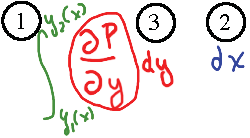
\includegraphics[width=1.2in]{figures/greedy_ex-2.pdf}
\captionsetup{font=footnotesize}
 \captionof{figure}{Without considering the semantics of these symbols and before the last stroke ($\frac{\delta p}{\delta y}dy$) is inserted, the first two strokes ($-\int^a_b$ and $dx$) appear like two separate equations with a large space between them.}
\label{fig:baselineinset}
}
For example, in
Figure~\ref{fig:baselineinset}, there is a large space between the first stroke ($-\int^a_b$, \raisebox{.5pt}{\textcircled{\raisebox{-.9pt} {1}}}) and the second stroke ($dx$, \raisebox{.5pt}{\textcircled{\raisebox{-.9pt} {2}}}). Without considering the semantics of these symbols, 
they appear to be separate equations. However, once we consider 
the subsequent set of red strokes(\raisebox{.5pt}{\textcircled{\raisebox{-.9pt} {3}}})
 it becomes clear that this is not the best segmentation. In general, computing good stroke segmentations requires considering
the global configuration of strokes in both space and time. \\

In this respect, the problem of segmenting strokes into visual
entities is analogous to the
\emph{line-breaking} problem, i.e., arranging the words of a paragraph
into lines.  In both cases, we want to segment a sequence of elements
(strokes or words) into an optimal set of groups (visual entities or
lines) defined by some scoring function over candidate entities or lines.
An important difference is that in the traditional line-breaking problem, only a
contiguous set of words can be put on the same line. In our case,
strokes in one visual entity can be interspersed by strokes in a
different visual entity. For example, the instructor may
go back and forth between two lines of equations, or
between a graph and an equation (Figure~\ref{Fig:line_order}).\\

Given these observations, we propose a dynamic programming approach for
stroke segmentation based on the classic optimal line-breaking
algorithm~\cite{knuth1981breaking} that handles non-contiguous grouping.
We first explain the high-level structure of the algorithm before
describing the scoring function in deta
%
\subsubsection{Algorithm Overview}
Figure \ref{Fig:pseudocode} gives a detailed pseudo-code of our segmentation algorithm.\\    
%
\begin{figure}[h!]
        \centering
        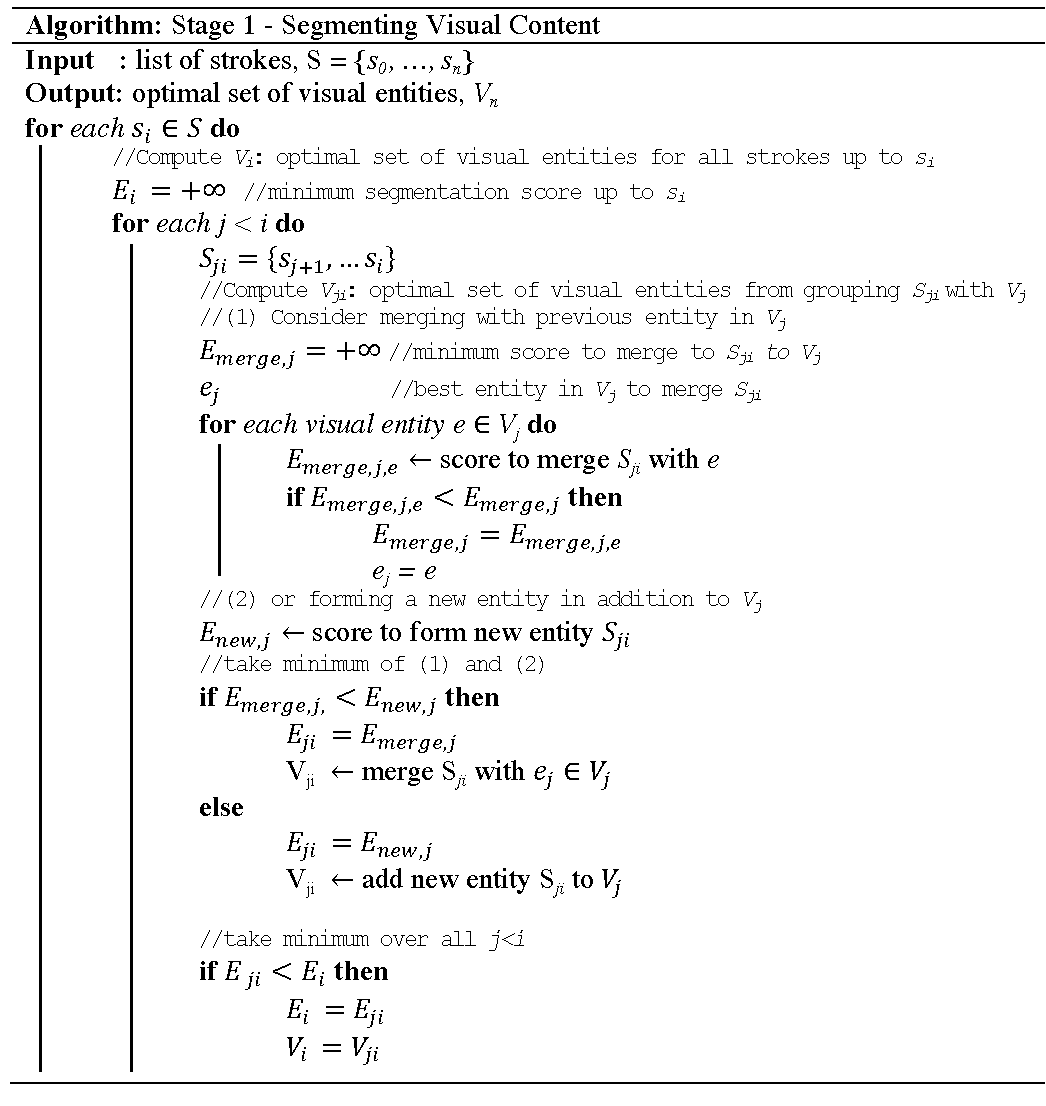
\includegraphics[width=\textwidth]{figures/pseudocode_image.pdf}
	\captionsetup{font=footnotesize}
        \caption{We use dynamic programming to segment strokes into an optimal
set of visual entities. For each stroke, $s_i$, the algorithm considers all previous
partial solutions, $V_{j<i}$ and $S_{ji}=\{s_{j+1}, ..., s_i\}$. For each
$V_j$, it considers two possibilities: merging $S_{ji}$ with an existing
entity or forming a new entity.}
        \label{Fig:pseudocode}
\end{figure}\\
%
Given a sequence of $n$ strokes $S = \{s_o,\dots,s_n\}$ ordered by
when they appear in the video, we find the optimal set of inter-stroke
boundaries that segment the strokes into visual entities. We refer to the boundary between $s_i$ and $s_{i+1}$ as
$b_i$.
%
Our algorithm processes the strokes in order and for each $s_i$
computes and records the optimal set of visual entities $V_i$ formed
by all strokes up to $b_i$, along with the total score $E(V_i)$ of
this partial solution.
%
To determine the optimal partial solution for stroke $s_i$, we
consider each previous boundary $b_j$ where
$\setlength{\thickmuskip}{0mu} j<i$, and evaluate two possible ways of
grouping the set of strokes $S_{ji} = \{s_\text{j+1},
\dots,s_\text{i}\}$: 1) merging $S_{ji}$ with one of the existing entities
in $V_j$, or 2) forming a new entity with $S_{ji}$. 
%
Allowing $S_{ji}$ to be merged with existing entities enables our
algorithm to support non-contiguous stroke groupings.
%
We take the better (lower) of the two scores for $S_{ji}$ and add it
to $E(V_j)$ to obtain the total score for the proposed
segmentation. After considering all candidate boundaries $b_j$, we
identify the partial solution with the minimum segmentation score and
record the corresponding set of entities as $V_i$ and the score as $E(V_i)$.
%
Once the algorithm iterates through all strokes, $V_n$ gives the
optimal set of visual entities for the entire lecture.
%
%
\subsubsection{Scoring Function}
The dynamic programming algorithm described above requires a scoring
function that evaluates the goodness of candidate visual entities
formed by sets of strokes. We define this scoring function based on
several observations: Strokes within a visual entity are (1) compactly arranged (2) and horizontally aligned. In addition, separate visual entities are (3) spatio-temporally distant from each other.
%

%----------------------------------------------------------------------------------------
\section{User Evaluation}
%----------------------------------------------------------------------------------------
\section{Discussion}